\let\negmedspace\undefined
\let\negthickspace\undefined
\documentclass[journal]{IEEEtran}
\usepackage[a5paper, margin=10mm, onecolumn]{geometry}
%\usepackage{lmodern} % Ensure lmodern is loaded for pdflatex
\usepackage{tfrupee} % Include tfrupee package

\setlength{\headheight}{1cm} % Set the height of the header box
\setlength{\headsep}{0mm}     % Set the distance between the header box and the top of the text

\usepackage{gvv-book}
\usepackage{gvv}
\usepackage{cite}
\usepackage{amsmath,amssymb,amsfonts,amsthm}
\usepackage{algorithmic}
\usepackage{graphicx}
\usepackage{textcomp}
\usepackage{xcolor}
\usepackage{txfonts}
\usepackage{listings}
\usepackage{enumitem}
\usepackage{mathtools}
\usepackage{gensymb}
\usepackage{comment}
\usepackage[breaklinks=true]{hyperref}
\usepackage{tkz-euclide} 
\usepackage{listings}
% \usepackage{gvv}                                        
\def\inputGnumericTable{}                                 
\usepackage[latin1]{inputenc}                                
\usepackage{color}                                            
\usepackage{array}                                            
\usepackage{longtable}                                       
\usepackage{calc}                                             
\usepackage{multirow}                                         
\usepackage{hhline}                                           
\usepackage{ifthen}                                           
\usepackage{lscape}

\begin{document}

\bibliographystyle{IEEEtran}
\vspace{3cm}

\title{2.4.5}
\author{EE25BTECH11015 - Bhoomika V}
% \maketitle
% \newpage
% \bigskip
{\let\newpage\relax\maketitle}

\renewcommand{\thefigure}{\theenumi}
\renewcommand{\thetable}{\theenumi}
\setlength{\intextsep}{10pt} % Space between text and floats


\numberwithin{equation}{enumi}
\numberwithin{figure}{enumi}
\renewcommand{\thetable}{\theenumi}
\parindent 0px 
{Question :-} \\ 

Show that the points 
$\vec{A}(2\hat{i} - \hat{j} + \hat{k}),\;
\vec{B}(\hat{i} - 3\hat{j} - 5\hat{k}),\;
\vec{C}(3\hat{i} - 4\hat{j} - 4\hat{k})$
are the vertices of a right angled triangle. \\ \\

\solution \\

\begin{table}[H]    
  \centering
  \begin{table}[h!]
    \centering
    \begin{tabular}{|c|c|}
        \hline
        Point & Coordinates \\
        \hline
	    $A$ & $\myvec{1\\-1}$ \\
	    $B$ & $\myvec{-4\\2k}$ \\
	    $C$ & $\myvec{-k\\-5}$ \\
        \hline
    \end{tabular}
    \caption{Vertices of $\triangle ABC$ before substituting $k$}
    \label{tab:triangle_k}
\end{table}

  \caption{Vectors}
  \label{Answers}
\end{table}


The sides of the triangle will be 
\begin{equation}
\vec{B}-\vec{A} = 
\begin{bmatrix}
-1 \\ 
-2 \\ 
-6
\end{bmatrix}, \quad
\vec{C}-\vec{B} = 
\begin{bmatrix}
2 \\ 
-1 \\ 
1
\end{bmatrix}, \quad
\vec{A}-\vec{C} = 
\begin{bmatrix}
-1 \\ 
3 \\ 
5
\end{bmatrix}
\label{1}
\end{equation}
 In a right angled triangle 
\begin{equation}
(\vec{C}-\vec{B})^{T} (\vec{A}-\vec{C}) = 0
\label{2}
\end{equation}

from Equation~\eqref{1}
\begin{equation}
(\vec{C}-\vec{B})^{T} (\vec{C}-\vec{A}) = \begin{bmatrix}
2 &-1  & 1
\end{bmatrix}\begin{bmatrix}
-1 \\ 
3 \\ 
5
\end{bmatrix}=0
\end{equation}

Therefore the given points are vertices of a right angled triangle.
\begin{figure}[H]
\begin{center}
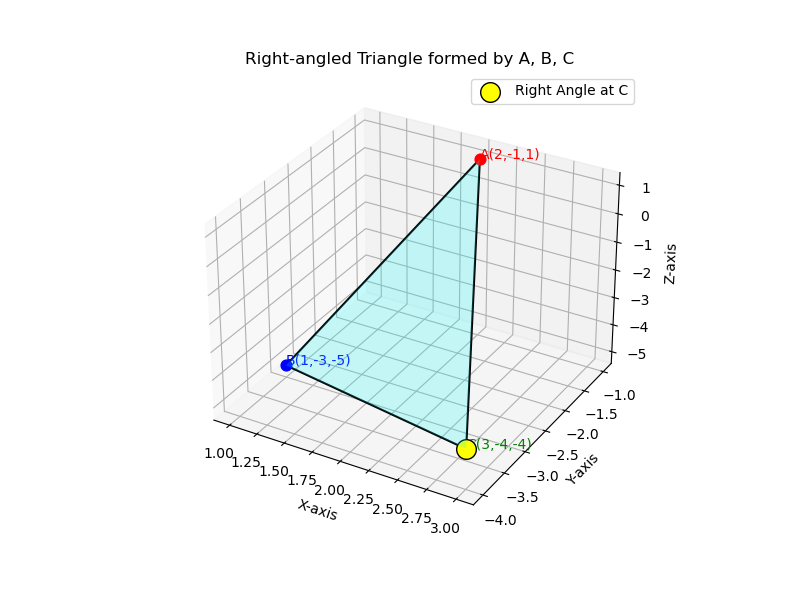
\includegraphics[width=0.6\columnwidth]{Figs/Fig1.png}
\end{center}
\caption{}
\label{fig:Fig.1}
\end{figure}

\end{document}
